\documentclass[12pt]{article}
\usepackage{hyperref}
\usepackage[letterpaper,left=1in,right=1in,top=1in,bottom=1in]{geometry}
\usepackage{setspace}
\usepackage{graphicx}
\usepackage{float}
\usepackage{listings}
\doublespacing
\usepackage{amsmath}
\lstset{
  basicstyle=\ttfamily,
  frame=single,
  breaklines=true,
}
\newcommand{\ignore}[1]{}
% im using the ubuntu package: "pdflatex" to compile this cause when I put pngs in it, that makes it easier
% hopefully that works for how you compile .tex files
\begin{document}
~\\
Scott Griffy \\
Robert Handy \\
Spring 2019 \\
CS545 - Machine Learning \\
Teacher: Anthony Rhodes \\
Assignment: Final Project Report \\
Title: Classifying malicious and benign binaries \\
Presented: June 10th, 2019 \\
\par
The EMBER dataset is a set of binaries.
The white paper can be found at: \url{https://arxiv.org/abs/1804.04637} and the code used to manipulate the dataset can be found at \url{https://github.com/endgameinc/ember}.
The dataset is designed to assist with training malware classifiers using machine learning to classify malicious binaries.
The dataset consists of a training set of 300K malware binaries, 300K benign binaries (binaries that do not have an adverse affect on computers), 300K unlabeled binaries (these could be either malicious or benign, it is not known which).
The dataset also includes a test set consisting of 100K malicious binaries and 100K benign binaries.
\par
Finding data to use for machine learning models that classify malware is a difficult task.
One of the problems in acquiring and publishing a dataset is licensing issues surrounding the binaries in the dataset.
Many binaries are not permitted for distribution because of commercial licenses.
The authors of the EMBER dataset avoided this by releasing features of binaries in place of the actual binaries.
\par
The authors of EMBER removed the actual binaries from this dataset.
This protects the researchers performing the machine learning algorithms.
If malicious binaries were included in the dataset, the researchers could potentially infect themselves while training a model.
\par
Another large contribution of the authors of the EMBER dataset is the labels of the binaries. Labeling binaries is difficult work, which is generally done by hand by experts. Because of this difficultly and level of skill required, a label indicating binaries as malware or benign is very valuable. This dataset contains 800K labeled binaries and their features.
\par
In our project, we used this dataset to train different machine learning models.
We used a Bayesian learning algorithm on the labeled data of the EMBER dataset, and a K-means algorithm on the unlabeled data. We compare these two models in the conclusion of this report.
\section{K-Means}
\par
The unlabeled data in the dataset is meant to be used for semi-supervised learning.
This was out of scope for this project as we did not learn about semi-supervised techniques in class.
Hopefully the unsupervised model we performed on the data (and the model's analysis) is interesting enough to be a significant contribution to understanding how the EMBER dataset can be used for machine learning models.
\par
We used the k-means algorithm to do unsupervised learning. A PCA dimensionality reduction was run on the data to reduce the features from 2351 to 2. This allows us to graph the data points in 2-D space.
The problem with running a fully unsupervised scheme rather than using a semi-supervised algorithm is that the unsupervised algorithm may find a different distinction than malicious or benign.
The k-means ended up getting 50\% accuracy on the test data, which, because the test data was evenly split, was just as good as guessing. The result of the training is shown in Figure \ref{fig:kmeans_training}.
After graphing the points retrieved from PCA and categorized with k-means it seemed that the k-means algorithm had strictly split the data along the x-axis.
\par
After graphing the test points and their classifications, we noticed that the y-axis actually did a much better job of separating the data. This is shown in Figure \ref{fig:kmeans_testing}.
Just using the y-axis as a classifier, and choosing a split based on the average y value of training points, we achieved an accuracy of 70\%.
An example run of the program is shown in Listing \ref{lst:prog}.
\begin{lstlisting}
$ python3 kmeans/kmeans.py 10000 5000
original # dimensions 2351
# unlabeled 10000
# pos 2500
# neg 2500
scaling...
pca-ing to  2  dimensions...
max args: - pca component vectors (out of 2351 features)
         1473
         509
training (kmeans on 2 centers)...
FOR DEBUGGING:
         label min 0
         label max 1
testing...
total 5000
correct 2557.0
accuracy 0.5114
confusion_matrix
 [[2426.   74.]
 [2369.  131.]]
totalEntropy - kmeans 0.8136407057087205

==Classifying using minor axis in 2 dim PCA==
meany 2.3874235921539365e-16
totalEntropy - pca1 0.7617772608209377
y eval (# correct,total) 3511 5000
y eval accuracy 0.7022
creating graphs
saving learning cluster to  ./kmeans_clusters.png
saving guess cluster to  ./kmeans_guesses.png
\end{lstlisting}

\begin{figure}[ht]
\centering
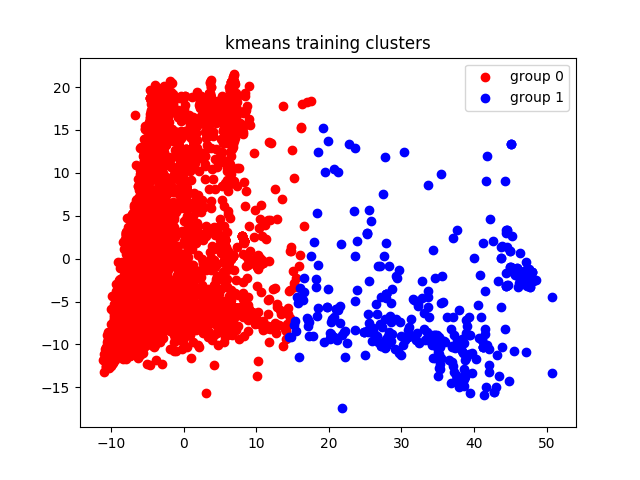
\includegraphics[width=.5\textheight]{kmeans_clusters}
\caption{k-means clusters after training}
\label{fig:kmeans_training}
\end{figure}
\begin{figure}[ht]
\centering
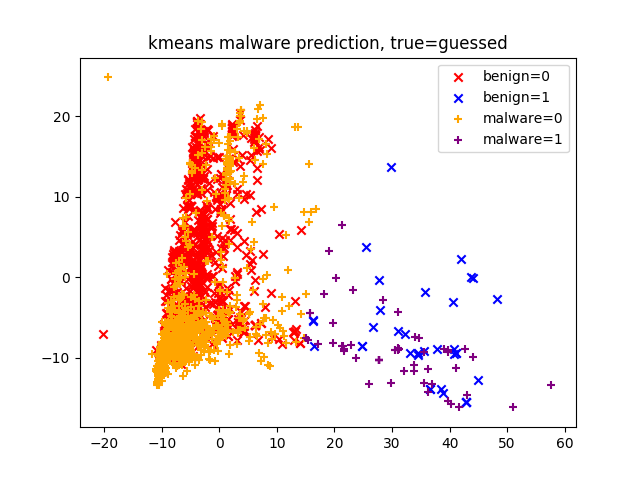
\includegraphics[width=.5\textheight]{kmeans_guesses}
\caption{k-means results after testing}
\label{fig:kmeans_testing}
\end{figure}
\section{Bayesian}
\par
We also used a Bayes Classifier to classify the labeled data. The Bayes algorithm was originally run on all 2351 features in the dataset. Running on 5000 test data points it produced about 60\% accuracy. The confusion matrix for this data can be seen in Table \ref{tab:bayes_all_features} (with the rows representing the actual values and the columns representing the predicted values): 
\begin{table}[]
    \centering
    \begin{tabular}{|c|c|c|}
        \hline
         & Not Malware & Malware  \\
         \hline
        Not Malware & 1037 & 1632 \\
        \hline
        Malware & 324 & 2007 \\
        \hline
    \end{tabular}
    \caption{Bayes All Features}
    \label{tab:bayes_all_features}
\end{table}

In order to determine why we get such poor results for a Bayes Classifier, we delved into the features and examined the differences between each feature for the malware and not malware. Figure \ref{fig:feature_distributions} shows the distributions for four different features for both the malware and not malware data. As is obviously clear, there is a lot of overlap between these features and so it is difficult for the Bayes Classifier to determine which class a particular datapoint belonged to. In order to combat this, we removed the features with the most overlap between the two classes, leaving only about 20 features of the original 2351 that had the most separation. Running a Bayes Classifier with only these features yielded far better results, improving the accuracy to about 80\% accuracy. This improved accuracy comes from essentially eliminating all of the "noise" that was injected into the Bayes Classifier with all of the features that were not easily distinguishable between the malware and not malware classes. The confusion matrix for the reduced features can be seen in Table \ref{tab:bayes_best_features}.



\begin{figure}[H]
\centering
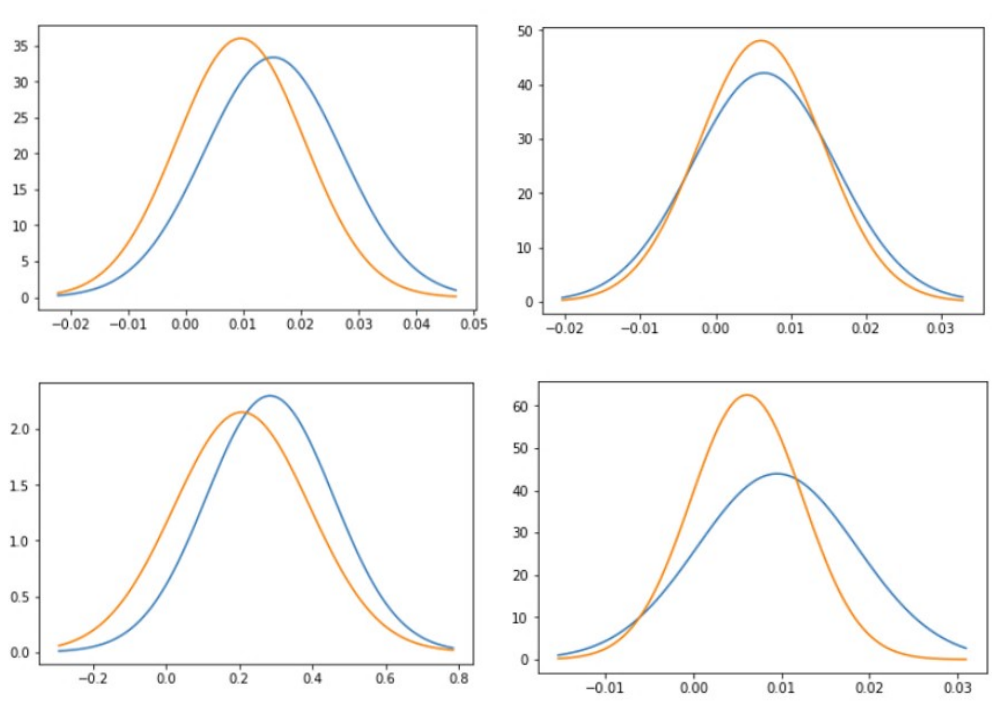
\includegraphics[width=.5\textheight]{Features}
\caption{Feature Distributions}
\label{fig:feature_distributions}
\end{figure}

\begin{table}[]
    \centering
    \begin{tabular}{|c|c|c|}
        \hline
         & Not Malware & Malware  \\
         \hline
        Not Malware & 1756 & 913 \\
        \hline
        Malware & 68 & 2263 \\
        \hline
    \end{tabular}
    \caption{Bayes Best Features}
    \label{tab:bayes_best_features}
\end{table}

\par
Interestingly, the Bayes Classifier tended to produce a large number of false positives. As can be seen in Table \ref{tab:bayes_all_features} and Table \ref{tab:bayes_best_features} the majority of the incorrectly classified data falls under the false positive section. This problem was exacerbated when we applied a PCA reduction in order to try and trim the features. Using a PCA reduction to 50 dimensions resulted in an accuracy of 54\%, hardly better than just making a random guess. The confusion matrix shown in \ref{tab:bayes_pca_reduction} shows that about 80\% of the not malware data was classified as malware. This trend continued for various numbers of dimensions that it was reduced to and it was thus determined that a PCA reduction is not useful for this dataset on a Bayes Classifier.

\begin{table}[]
    \centering
    \begin{tabular}{|c|c|c|}
        \hline
         & Not Malware & Malware  \\
         \hline
        Not Malware & 533 & 2136 \\
        \hline
        Malware & 186 & 2145 \\
        \hline
    \end{tabular}
    \caption{Bayes PCA Reduction - 50 Dimensions}
    \label{tab:bayes_pca_reduction}
\end{table}
\section{Conclusion}
\par
After running experiments on the EMBER dataset, we found interesting results. It seems that Bayesian learning performed much better than k-means. This can be seen by comparing their accuracy. Both strategies needed to be tweaked to perform well.
Both strategies found dimensionality reduction to be very important. Bayesian seemed to need hand picked dimensions from the dataset, and for k-means, simple PCA performed better.
\par
The largest failure of the dataset is the inability of the EMBER code to reverse the vectorized features back into raw features. Because of this, we cannot extrapolate our finding to say anything about the features of malware such as byte frequency or header imports. We can test the viability of different machine learning model.
Hopefully more models can be trained on this dataset leading to more discoveries about the nature of malware classification.
\end{document}
